
    La liste est une collection ordonnée et modifiable. Elle autorise la duplication des items.
    
    Le tuple est une collection ordonnée et immuable. Permet la duplication des items.
    
    Set est une collection non ordonnée, non modifiable et non indexée. Pas d'items en double.
    
    Dictionnaire : collection ordonnée et modifiable. Pas d'items en double.
\subsection{Lists}

\textbf{Les éléments de la liste sont ordonnés, modifiables et peuvent être dupliqués.}

Pour manipuler une liste, ouvrez un éditeur de texte et
écrivez :

\lstinputlisting[language = python]{chapitre2/codes/liste.py}

La sortie écran obtenue est la suivante : 

\begin{figure}[H]
    \centering
    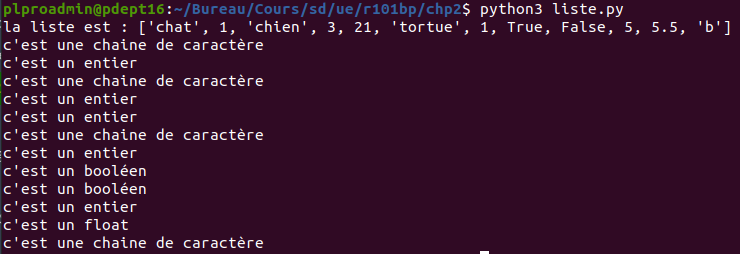
\includegraphics[scale = 0.7]{chapitre2/figures/liste1.png}
\end{figure}

\begin{tcolorbox}[lefttitle=2cm, colframe=gray!75!blue, title= \textbf{Tip for Code 1 : "\textit{Pour un code svelte et en bonne santé}"}]

Votre code commence à prendre de la place.

Par convention, la largeur maximale d'une ligne est de 79 charactères.

Le caractère $\backslash$ permet de couper des lignes trop longues. 

\url{https://peps.python.org/pep-0008/#maximum-line-length}

\end{tcolorbox}


\begin{tcolorbox}[lefttitle=2cm, colframe=gray!75!black, title= \textbf{Exercices}]
\textbf{1$\diamondsuit$-}
Complétez le programme suivant de façon à affecter trois listes : listeChaine, listeBool, listeInt, listeFloat, et listeAutres.
Afficher ces listes de façon à générer la sortie terminale suivante.

\begin{figure}[H]
    \centering
    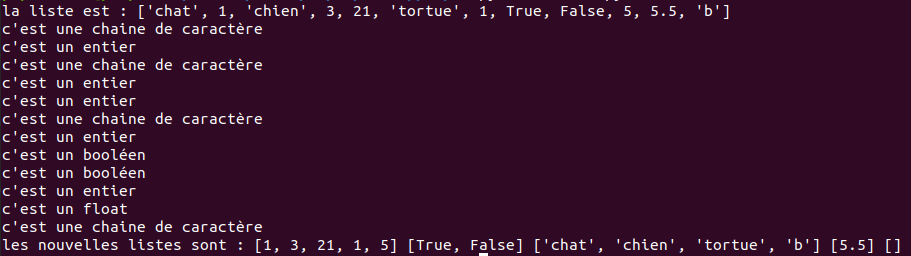
\includegraphics[scale=0.47]{chapitre2/figures/liste2.png}
\end{figure}


\textbf{2$\diamondsuit$-}
Modifiez le programme afin de ranger par ordre croissant listeEntier.

Modifiez le programme afin d'inverser listeChaine.

\textbf{Aide} : \url{https://www.w3schools.com/python/python_lists_methods.asp}

\textbf{(optionnel)3$\diamondsuit~\diamondsuit$-}
Modifiez le programme afin d'afficher une liste qui contient l'avant-dernier éléments de chacune des listes (ou rien si la liste est plus petite).

Et afficher une valeur au hasard de cette liste.

\textbf{Aide} : random.choice(maListe) \url{https://docs.python.org/3/library/random.html}


\end{tcolorbox}

\subsubsection{Strings}

Les strings sont des listes un peu particulières\footnote{\url{https://www.w3schools.com/python/python_strings_methods.asp}}.

Ouvrez un éditeur de texte et écrivez :

\lstinputlisting[language = python]{chapitre2/codes/string.py}

La sortie écran que vous devez obtenir est la suivante : 

\begin{figure}[H]
    \centering
    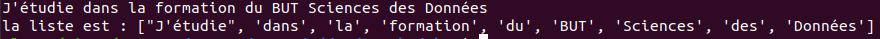
\includegraphics[scale = 0.5]{chapitre2/figures/string.png}
\end{figure}

\begin{tcolorbox}[lefttitle=2cm, colframe=gray!75!blue, title= \textbf{Tip for Code 2 : "\textit{Les expressions régulières}"}]

\begin{figure}[H]
    \begin{minipage}[c]{0.4\textwidth}
    Réservée aux plus aguerris, une expression régulière ou regex est une chaîne de caractères qui décrit, selon une syntaxe précise, un ensemble de chaînes de caractères possibles.

    Il existe sur internet des petits jeux pour apprendre à les maîtriser comme \url{https://regexcrossword.com/}.
    \end{minipage}\hfill
    \begin{minipage}[c]{0.5\textwidth}
    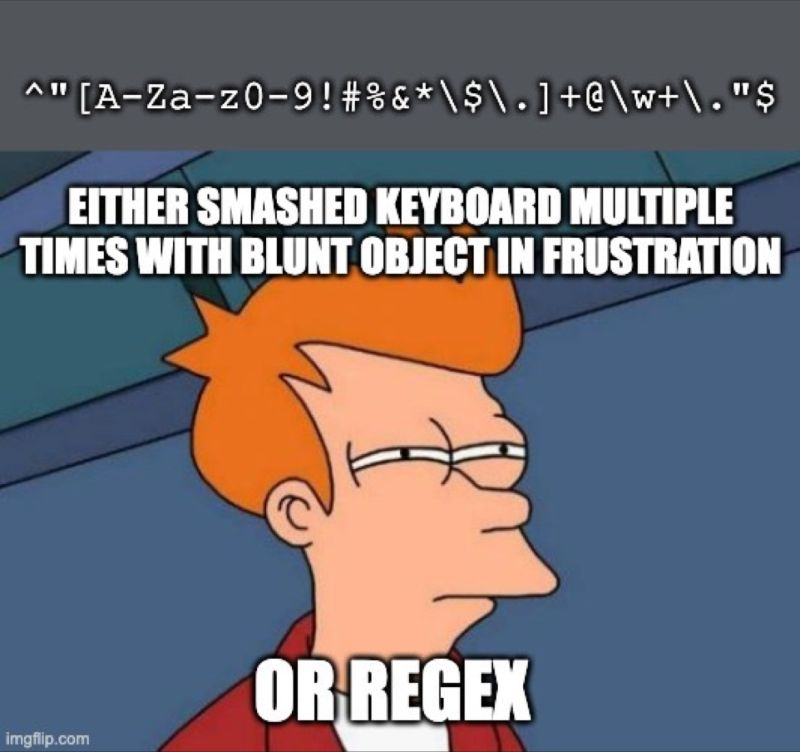
\includegraphics[scale=0.27]{chapitre2/figures/regex.jpeg}
    \end{minipage}
\end{figure}

\end{tcolorbox}



\begin{tcolorbox}[lefttitle=2cm, colframe=gray!75!black, title= \textbf{Exercices}]
\textbf{1$\diamondsuit$-}
Complétez le programme suivant de façon à partir de la liste finale :

\begin{enumerate}
    \item Affichez le nombre de mots de la liste
    \item Affichez le nombre d’occurrences du mot "BUT"
    \item Rajouter entre "J'étudie" et "dans" les éléments "à", "Dole"
    \item Supprimer les deux derniers éléments de la liste
    \item Rajouter des "euh" à chaque espace 
\end{enumerate}

Puis, recréez une phrase (sctring) à partir de cette liste et affichez là.
Le résultat devrait être ainsi :
\begin{figure}[H]
    \centering
    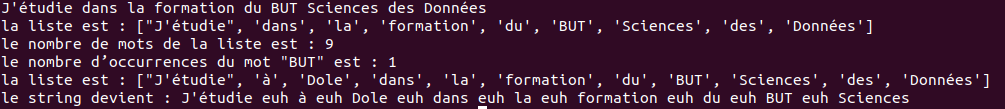
\includegraphics[scale = 0.4]{chapitre2/figures/string2.png}
\end{figure}


\textbf{2$\diamondsuit$-}
Complétez le programme suivant de façon à partir d'un string obtenu

\begin{enumerate}
    \item mettez le string en majuscule (aide : upper()\footnote{\url{https://www.geeksforgeeks.org/python-string-upper/}})
    \item remplacez les "euh" par un espace " " (aide : replace() )
    \item afficher si le string contient le mot "DOLE" (aide : rfind())
\end{enumerate}

Puis, recréez une liste à partir de ce string et affichez là en minuscule.

\textbf{(Optionnel)3$\diamondsuit~\diamondsuit~\diamondsuit$-}
Modifier la comparaison avec "DOLE" de façon à ce qu'elle soit insensible à la case.

\end{tcolorbox}



\subsection{Tuples}

\textbf{Les éléments d'un tuple sont ordonnés, immuables et peuvent être dupliqués.}
En mathématiques, on parle de p-uplets, avec $p$ ne nombre d'éléments \url{https://python-reference.readthedocs.io/en/latest/docs/tuple/}. 


Ouvrez un éditeur de texte et écrivez :

\lstinputlisting[language = python]{chapitre2/codes/tuple.py}

La sortie écran que vous devez obtenir est la suivante : 

\begin{figure}[H]
    \centering
    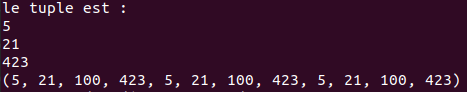
\includegraphics[scale = 0.5]{chapitre2/figures/tuple.png}
\end{figure}


\begin{tcolorbox}[lefttitle=2cm, colframe=gray!75!black, title= \textbf{Exercices}]
\textbf{1$\diamondsuit$-}
Complétez le programme précédent de façon à fournir :

\begin{enumerate}
    \item la somme des dépenses
    \item la dépense la plus importante
    \item la dépense la moins importante
    \item le nombre de loyers payés (montant 423)
    \item le nombre de dépenses
    \item la moyenne des dépenses
    \item la somme des dépenses
\end{enumerate}

L'affichage termianl obtenu devrait être le suivant :

\begin{figure}[H]
    \centering
    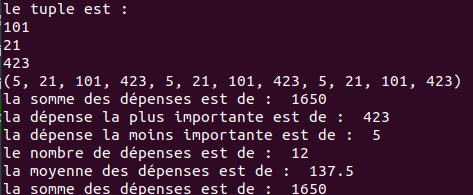
\includegraphics[scale = 0.6]{chapitre2/figures/tuple2.png}
\end{figure}

Aide : \url{https://python-reference.readthedocs.io/en/latest/docs/tuple/}

\end{tcolorbox}


\begin{tcolorbox}[lefttitle=2cm, colframe=gray!75!blue, title= \textbf{Tip for Code 3 : psychologie d'un tuple}]

Les tuples étant non modifiables, que se passe-t-il alors avec un tuple contenant des objets modifiables comme des listes ? 
\begin{figure}[H]
    \begin{minipage}[c]{0.53\textwidth}
Analyse du code suivant code suivant :
\lstinputlisting[language = python]{chapitre2/codes/tupleAvecListe2.py}

    \end{minipage}\hfill
    \begin{minipage}[c]{0.45\textwidth}

Il existe deux grands types de copie :
\begin{itemize}
    \item La copie par valeur recrée un objet identique. Deux objets d'adresse différente mais de valeur identique sont créés.
    \item La copie par référence copie l'adresse (ou référence) de l'objet. Il n'existe donc qu'un seul objet.
\end{itemize}

    \begin{center}
    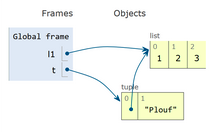
\includegraphics[scale=0.7]{chapitre2/figures/memoire.png}    
    \end{center}
    
    
La liste l1 pointe vers le même objet que l'élément du tuple d'indice 0. C'est une copie par référence (même adresse).
Donc, Dans notre cas, le premier élément du tuple pointe vers une liste modifiable. 

    \end{minipage}
\end{figure}

\end{tcolorbox}




\subsection{Sets}

\textbf{Les éléments de l'ensemble sont non ordonnés, non modifiables et n'autorisent pas les valeurs en double.}

Pour manipuler un ensemble, ouvrez un éditeur de texte et
écrivez :

\lstinputlisting[language = python]{chapitre2/codes/ens3.py}

La sortie écran obtenue est la suivante : 

\begin{figure}[H]
    \centering
    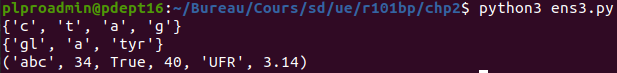
\includegraphics[scale = 0.7]{chapitre2/figures/ens3.png}
\end{figure}

\begin{tcolorbox}[lefttitle=2cm, colframe=gray!75!blue, title= \textbf{Tip for Code 4 : "\textit{Les duplications dans les ensembles}"}]

Les ensembles ne peuvent pas comporter deux éléments ayant la même valeur.
Les valeurs en double seront ignorées.
Le programme suivant :
\lstinputlisting[language = python]{chapitre2/codes/ens.py}
donnera la sortie écran suivante :


\begin{figure}[H]
    \centering
    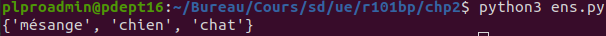
\includegraphics[scale = 0.7]{chapitre2/figures/ens.png}
\end{figure}

A votre avis, que donnera le programme suivant ?

\lstinputlisting[language = python]{chapitre2/codes/ens2.py}




\end{tcolorbox}


\begin{tcolorbox}[lefttitle=2cm, colframe=gray!75!black, title= \textbf{Exercice}]
\textbf{1$\diamondsuit$-}
A l'aide du programme précédent et de votre ordinateur, complétez le tableau suivant


\textbf{set}

\begin{tabular}{|l|c|}
    \hline   Instructions &  ~~~~~~~~~~~~~~~~~~~~~~~~~~~~~~~~~~~~~~~~~~~~Sortie écran ~~~~~~~~~~~~~~~~~~~~~~~~~~~~~~~~~~~~~~~~~~~~\\\hline
     $s = \{3, 4, "Plouf", (1, 3)\}$ & \\
     $print(s)$ &  \\\hline
      $s2 = \{3.14, [1, 2]\}$ & \\
     $print(s)$ &  \\\hline
       $print((set((2, 2, 2, 1))))$& \\\hline
      $s3 = set("BUT SD S1")$ &  \\ 
       $print(s3)$&\\\hline
      $s3.add(1)$ &  \\ 
       $print(s3)$&\\\hline
      $s3.discard('1')$ &  \\ 
       $print(s3)$&\\\hline
      $s3.discard('t')$ & \\ 
       $print(s3)$&\\\hline
      $print(s3.intersection(s))$&\\\hline
\end{tabular}


\end{tcolorbox}


\begin{tcolorbox}[lefttitle=2cm, colframe=gray!75!blue, title= \textbf{Tip for Code 5 : Etre ou ne pas être (hashable)}]

Commençons avec un rappel de vocabulaire :

\textbf{Un objet mutable} est ainsi un objet qui peut être modifié, dont on peut changer les propriétés une fois qu’il a été 
défini.\footnote{\url{https://docs.python.org/3/glossary.html\#term-mutable}}


A l'inverse, \textbf{un objet hashable} ne peut être modifié une fois qu’il a été 
défini.\footnote{\url{https://docs.python.org/3/glossary.html\#term-hashable}}

Les sets ne peuvent contenir que des objets hachables. Avoir des objets hashables optimise l'accès à chaque élément du set. Les objets hachables sont les chaînes de caractères, les tuples, les entiers, les floats, les booléens et les frozensets. Les objets non hachables que l'on connait sont les listes, les sets et les dictionnaires. 

\end{tcolorbox}






\subsection{Dictionaires}


Les dictionnaires permettent de manipuler des structures complexes. \textbf{Les dictionnaires sont des collections non ordonnées d'objets}. Il s'agit d'objets correspondance (mapping objects en anglais) ou tableaux associatifs. En effet, dans un même dictionnaire chaque valeur d'objet est accessible par une clé.


Pour manipuler un ensemble, ouvrez un éditeur de texte et
écrivez :

\lstinputlisting[language = python]{chapitre2/codes/dict.py}

La sortie écran obtenue est la suivante : 

\begin{figure}[H]
    \centering
    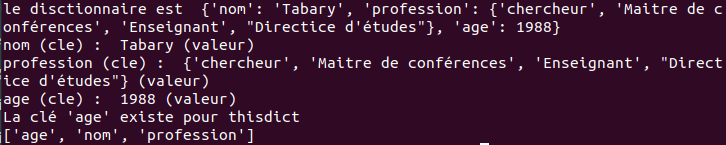
\includegraphics[scale = 0.7]{chapitre2/figures/dict.png}
\end{figure}


\begin{tcolorbox}[lefttitle=2cm, colframe=gray!75!black, title= \textbf{Exercice}]
\textbf{1$\diamondsuit$-}
Modifier le code précédent afin d'enlever la valeur enseignant chercheur au dictionnaire.

\textbf{2$\diamondsuit~\diamondsuit$-}
Rajouter le dictionnaire suivant au code

\begin{figure}[H]
    \centering
    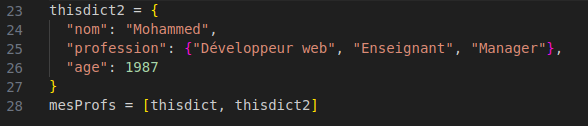
\includegraphics[scale = 0.7]{chapitre2/figures/dict2.png}
\end{figure}

\begin{itemize}
    \item affichez les noms de vos professeurs grâce à une boucle
    \item affichez l'ensemble des professions communes aux deux professeurs
\end{itemize}




\end{tcolorbox}


\subsection{Projets (optionnels)}


La recherche dichotomique prend en entrée une liste triée  \textit{T} et un élément \textit{v}.
Elle donne en résultat l'index, tel que \textit{T[index] = v}.
\subsubsection{Recherche simple}

On procède comme suit :
\begin{itemize}
    \item On compare v à chaque élément de la liste
    \item S’il est égal à v, on a fini
    \item Sinon, on prend l'élément suivant
    \item S’il est supérieur, on affiche l'information "pas d'éléments" sur le terminal
\end{itemize}

Donnez une preuve de terminaison, et la complexité de ce programme.


\textbf{Programmez un algorithme de recherche dichotomique.
}


\subsubsection{Recherche dichotomique}

On procède comme suit :
\begin{itemize}
    \item On compare v à l’élément du milieu de la liste.
    \item S’il est égal à v, on a fini.
    \item Sinon, s’il est inférieur, il faut chercher dans la première moitié de la liste. On retourne à l’étape 1 avec la liste réduite.
    \item S’il est supérieur, on fait de même avec la seconde moitié de la liste.
\end{itemize}

\textbf{Programmez un algorithme de recherche dichotomique.
}

Donnez une preuve de terminaison, et la complexité de ce programme.

\newpage

\subsection{Bilan (obligatoire)}



\makebox[0.75\textwidth]{Lors de ce TP, vous vous êtes arrêté à quel exercice ? \enspace\hrulefill}


\makebox[1\textwidth]{--------------------------------------------------Remplir le tableau--------------------------------------------------}

\textbf{Partie savoir faire}
\begin{itemize}
    \item Niveau 1 : Je n'ai pas su l'implémenter. C'est du charabiah pour moi. 
    \item Niveau 2 : J'ai lu le sujet. Les couleurs sont jolies. J'ai fini le premier exercice les yeux rivés sur mon clavier pour chercher les touches. Les erreurs de l'interpréteur me semblent incompréhensibles.
    \item Niveau 3 : J'ai pu avancer à la moitié du sujet, même si c'est difficile et que l'ordi est farceur (comme tous les ordis). Je prends beaucoup de temps à comprendre les erreurs du shell, mais j'y arrive !
    \item Niveau 4 : J'ai complété le TP avec aisance. La plupart des erreurs du shell me sont compréhensibles.
    \item Niveau 5 : J'ai complété le TP, exercices optionnels compris ! J'ai une grande agilité\footnote{agilité $\rightarrow$ ne pas utiliser la souris en codant} quand je code. 
\end{itemize}


\textbf{Partie savoir être}
\begin{itemize}
    \item Niveau 1 :  Pour finir au plus vite, j'élabore des stratégies (copier directement la réponse ou chercher à camoufler le désintérêt : "Si je n'y arrive pas, c'est que le prof n'est pas venu assez vite me donner la solution"). 
    \item Niveau 2 : L'objectif est d'avoir la moyenne sans trop y laisser du temps ou de l'énergie. Je suis bien obligé de faire le TP, même si l'idée de me servir du pannel de ressources me semble saugrenue. Si c'est possible de récupérer la réponse (ou de suivre à côté d'un camarade\footnote{Mais si, c'est du travail d'équipe : il code et je le soutiens émotionnellement !}), alors je ne dirai pas non. 
    \item Niveau 3 : Je prends doucement mes marques. Je me suis servi de façon hésitante de plusieurs ressoures dispos (shell, camarades, enseignants, manuel, sites web, ou même canard\footnote{\url{https://fr.wikipedia.org/wiki/M\%C3\%A9thode_du_canard_en_plastique}}) en cherchant à comprendre leur réponse. J'aimerais un jour pouvoir développer  mes propres projets et il faut pour cela que je gagne en autonomie.
    \item Niveau 4 :   Je suis autonome dans l'utilisation des ressoures disponibles (shell, camarades, enseignants, manuel, sites web, ou même canard\footnotemark[7]). J'ai même un projet personnel en cours que j'aimerais finir.
    \item Niveau 5 : J'évolue avec aisance dans cet environnement ! Je  fais même partie dorénavant des ressoures dispos et  j'échange facilement sur ces notions. J'ai plusieurs projets informatiques personnels. 
\end{itemize}

\begin{table}[H]
    \centering
    \begin{tabular}{|c|c|c|} \hline
        \textbf{Notions} & \textbf{Niveau atteint} (de 1 à 5) \textbf{Savoir faire}  & \textbf{Niveau atteint} (de 1 à 5) \textbf{Savoir être}\\\hline
        Liste & & \\\hline
        Tuple &&\\\hline
        Set &&\\\hline
        Dictionnaire &&\\\hline
        Respect des règles de bon codage && \\\hline
    \end{tabular}
\end{table}


